
\subsubsection{Electric polarizability $\alpha_E$ including all diagrams in the 1-window analysis}
\label{3571wAll}

%%%%%%%%%%%%%%%%%%%%%%%%%%%%%%%%%%%
\begin{figure}[H]
\centering
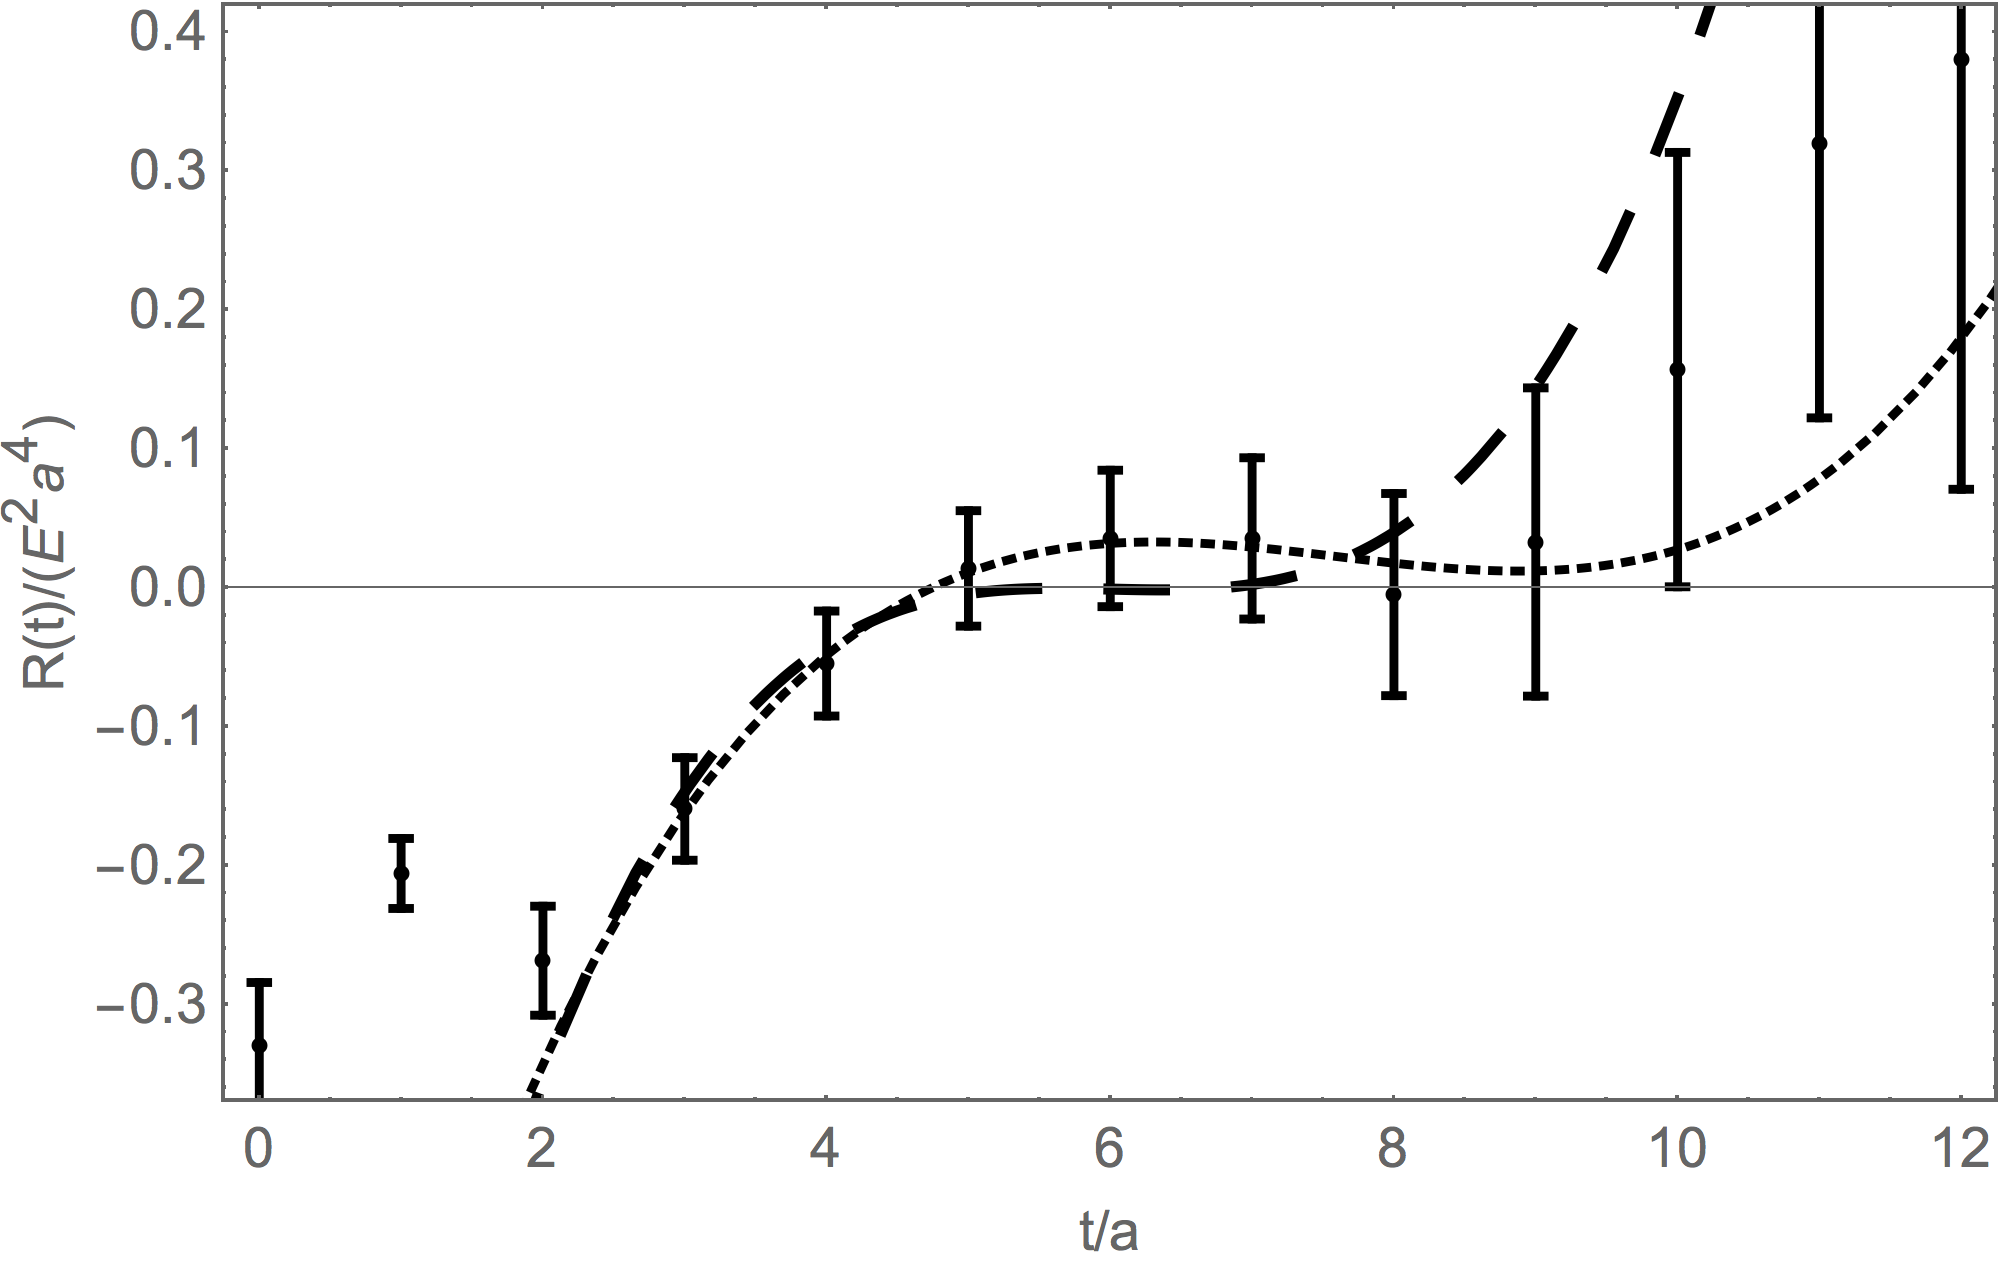
\includegraphics[width=.65\linewidth]{figures/shshQuadCSFull.png}\\
\caption{Correlator ratio $R_2(t)$ for all diagrams (connected and disconnected) shown in Figure ~\ref{fig:diagrams}, in units of $E^2a^4$. A cubic form was fitted with (dotted line) and without (dashed line) a quadratic term.}
\label{fig:1walphafull}
\end{figure}

%%%%%%%%Table 1-window full Multi point%%%%%%%%%
\begin{table}[H]
\begin{center}
    \begin{tabular}{ | l | l | l | }
    \hline
     Fit range [$t/a$]   			& 4 to 8   & 3 to 9  \\ \hline
     Inflection point [$t/a$]		& 12(55)   & 7.6(2.0)    \\ 
     						& 6.4(2.0)	& 7(82) \\\hline
     Extremal slope with   		&  -0.10(97)  &  -0.012(38) \\
     a quadratic term [$a^3$]	& 0.012(60) & 0.01(23) \\ \hline
     Extremal slope w/o		&  -0.000(25)   &  -0.002(22) \\
     a quadratic term [$a^3$]	& 0.011(60) & 0.005(53) \\ \hline
    \end{tabular}
\end{center}
\caption{Inflection points and extremal slopes for the $\chi^2$ cubic fits in the 1-window analysis for all connected and disconnected diagrams. \todo{results from reduced statistics are given in the lower lines}}
\label{tab:1walphafull}
\end{table}
%%%%%%%%%%%%%%%%%%%%%%%%%%%%%%%%%%%

%%%1-w polarizabilities goes here%%%
%%%%%%%%%Static polarizability 1-window Multipoint%%%%%%%%%%%%%%%
\begin{table}[H]
\begin{center}
    \begin{tabular}{|l||c|c||c|c||}
    \hline	& \multicolumn{2}{c}{with quadratic term} & \multicolumn{2}{c}{w/o quadratic term} \\ \hline
     Fit range [$t/a$)]						& 4 to 8 	& 3 to 9 	& 4 to 8 	& 3 to 9 \\ \hline 
     $\alpha_E$ [$10^{-4}$ $\text{fm}^3$]    		& 4(37)	& 0.5(1.4) 	& 0.01(94)	& 0.09(83) \\ \hline     
     $\alpha_E-\alpha_{FW}$ [$10^{-4}$ $\text{fm}^3$]& 4(37)	&  0.7(1.4)	& 0.23(94)	& 0.31(83) \\ \hline
    \end{tabular}
\end{center}
\caption{Static electric polarizability  $\alpha$ and reduced by the Foldy-Wouthuysen contribution $\alpha-\alpha_{FW}$ from the extremal values (1-window analysis, connected and disconnected diagrams, $\chi^2$ fits) of the two fit ranges in units of $10^{-4}$ $\text{fm}^3$. \todo{point results?}}
\label{tab:1wElectricPolarizabilityAllMultiPoint}
\end{table}
%%%%%%%%%%%%%%%%%%